% ============================================================
\section{Numerical Experiments}
\label{sec:experiments}
We evaluate the proposed physics-informed hybrid search(PIHS)
in cluttered environments containing both movable 
and immovable obstacles. All components—W-CCG presearch, frontier extraction, 
and the \textit{ModeTable} prior—are integrated as described in Sec.~\ref{sec:solution}. 
The implementation is in \texttt{Python~3}; 
simulations run in \texttt{PyBullet}~\cite{coumans2019} on a laptop with an Intel Core i7\textendash1280P CPU. 
Videos and logs are provided in the supplementary material.




% ========================================
\begin{table}[t]
  \centering
\begin{threeparttable}
  \caption{Performance on the nominal scenario with push-count (mean $\pm$ std).}
  \label{tab:main}
  \vspace{2pt}
  \setlength{\tabcolsep}{2.3pt}
\begin{tabular}{lccccc}
\toprule
Method & Succ.~(\%) & \#PT (s) & \#ET (s) & \#Sims & \#Pushes \\
\midrule
DFS-WCCG            & 25.0  & 41.8  & N/A     & --    & --   \\
SL-Push (off-line)  & 62.5  & 0.03  & 145.1   & 0.0   & 7.0  \\
SL-Push (sim)       & 75.0  & 25.1  & 246.8   & 16.0  & 8.0  \\
Rec-NAMO            & 37.5  & 10.5  & 179.3   & 0.0   & 7.0  \\
\textbf{PIHS (ours)}& \textbf{92.5} & \textbf{10.3} & \textbf{28.6} & \textbf{121.5} & \textbf{6.0} \\
\bottomrule
\end{tabular}
  \begin{tablenotes}[flushleft]\footnotesize
  \item \textbf{Metrics.} \emph{Succ.} = success rate; \emph{\#PT} = planning time; \emph{\#ET} = execution time; \emph{\#Sims} = simulations invoked; \emph{\#Pushes} = length of executed push sequence.
  \end{tablenotes}
  \end{threeparttable}
  \vspace{-4mm}
\end{table}

% ========================================
\begin{table}[t]
\centering
\caption{Ablations on the nominal scenario (40 trials).}
\label{tab:ablation}
\vspace{2pt}
\setlength{\tabcolsep}{3pt}
\renewcommand{\arraystretch}{0.95}
\begin{tabular}{lcccc}
\toprule
Variant & Succ.~(\%) & Time (s) & \#Sims & \#PT / \#Sims / Succ. \\
\midrule
SiLS (full)          & 92.5 & 28.6 & 122 & baseline \\
w/o presearch        & 85.0 & 35.2 & 178 & +6.6 / +56 / $-7.5$\% \\
w/o ModeTable        & 80.0 & 33.4 & 164 & +4.8 / +42 / $-12.5$\% \\
w/o quick-pass       & 90.0 & 41.9 & 208 & +13.3 / +86 / $-2.5$\% \\
w/o reinsertion      & 82.5 & 31.1 & 151 & +2.5 / +29 / $-10.0$\% \\
\bottomrule
\end{tabular}
\end{table}
% ========================================
\begin{figure}[t!]
  \centering
  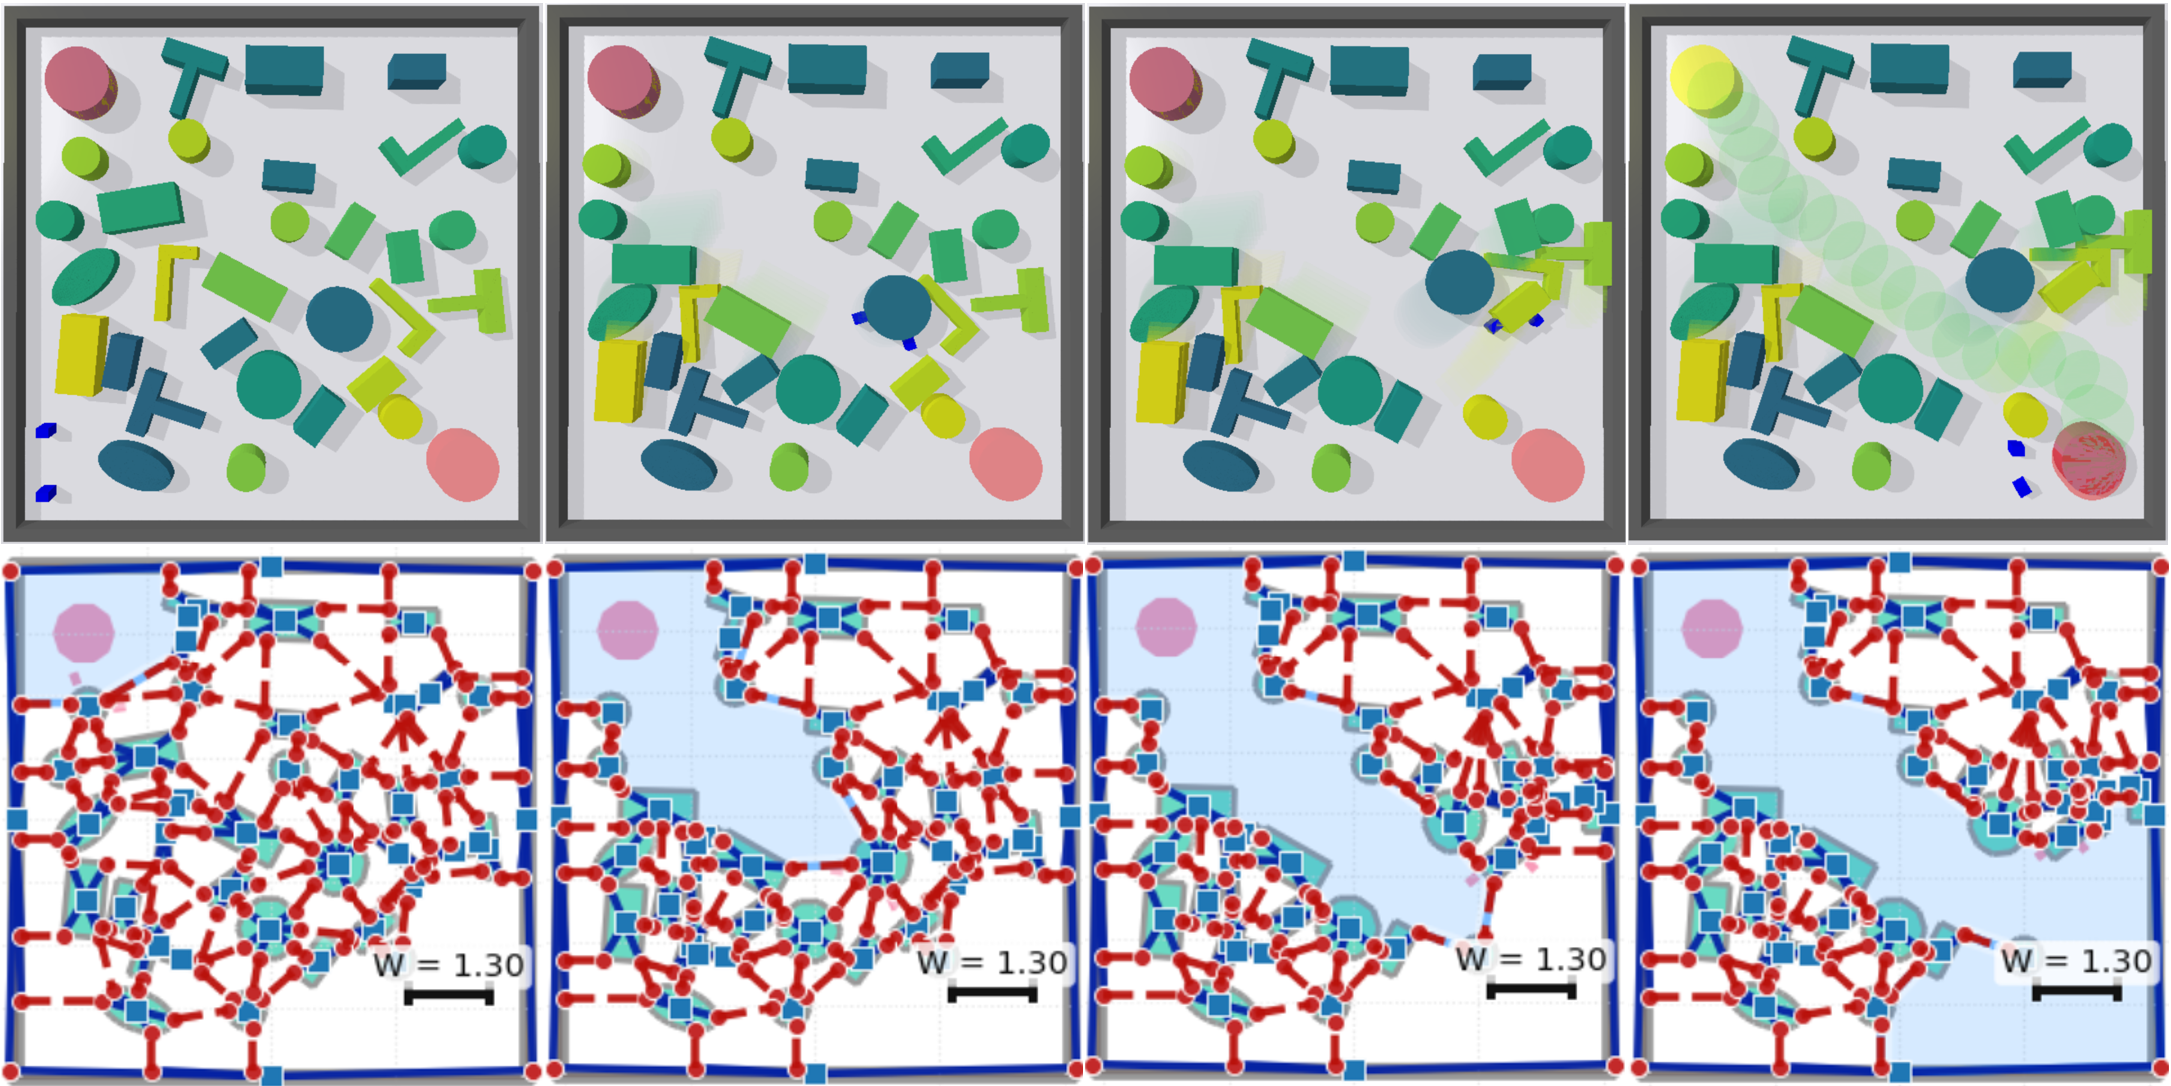
\includegraphics[width=0.95\linewidth]{figures/scalability.png}
  \vspace{-2mm}
 \caption{Scalability in dense clutter ($\boldsymbol{30}$ movables). 
  \textbf{Top:} four execution snapshots as the robots clear bottlenecks and advance toward the goals. 
  \textbf{Bottom:} corresponding WCCG overlays with the active face (translucent blue) and ranked gaps. 
  }
\label{fig:scalability}
\vspace{-4mm}
\end{figure}

\subsection{Numerical Simulations}
\label{subsec:sim}
% ========================================
% ========================================
\begin{figure*}[t]
  \centering
  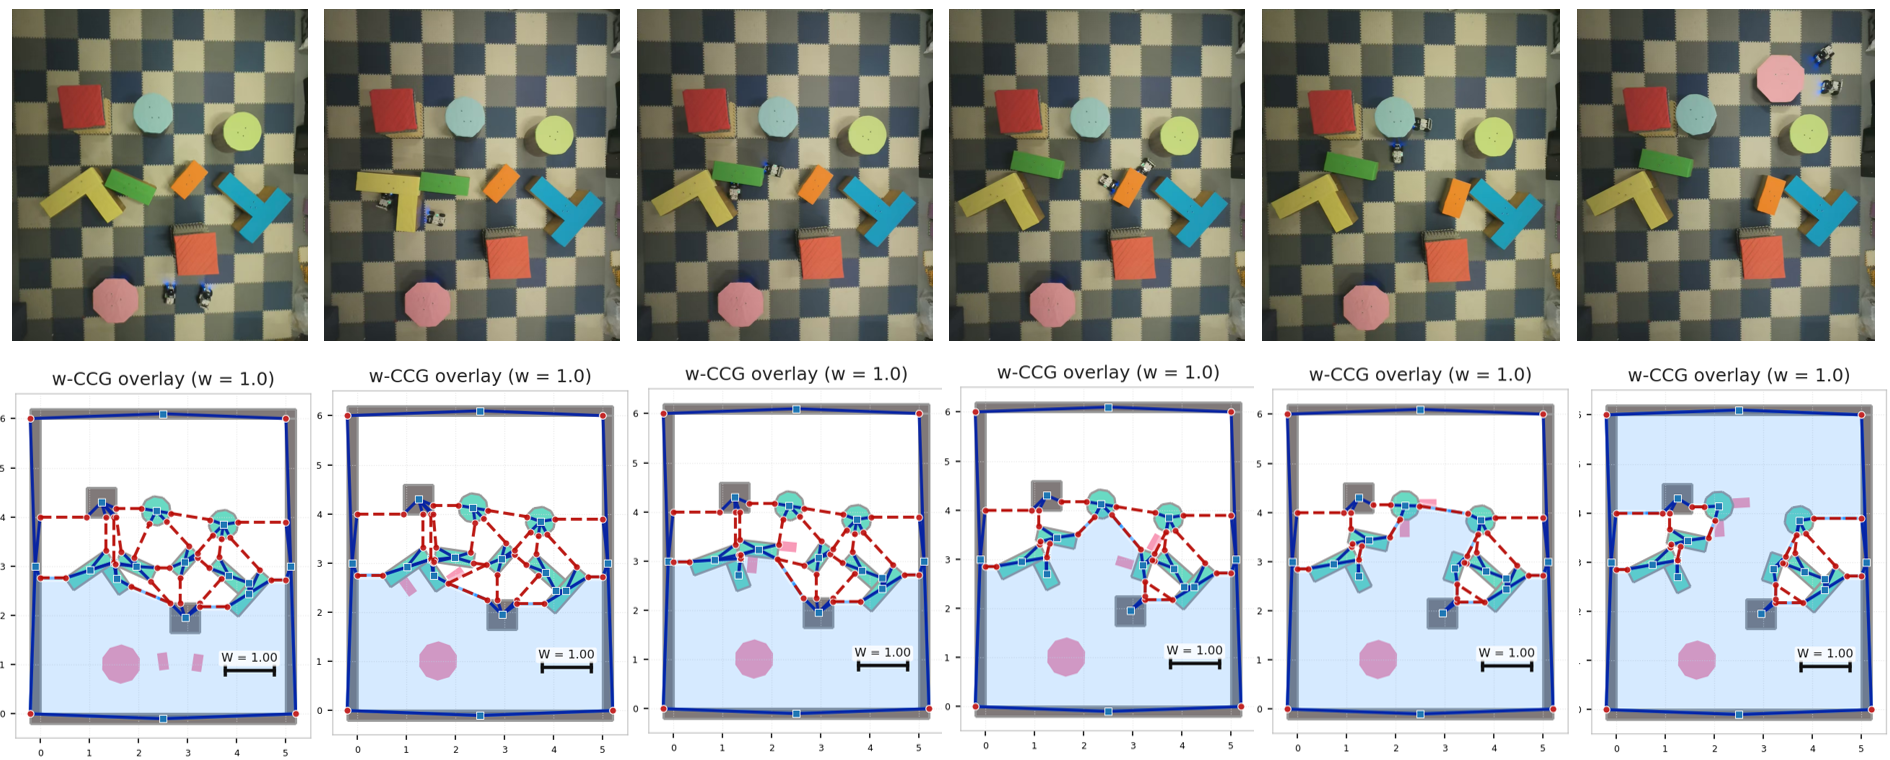
\includegraphics[width=0.95\linewidth]{figures/hardware_wccg.png}
  \vspace{-4mm}
  \caption{Real-world pushing experiment with execution--planning alignment. \textbf{Top:} six snapshots as two robots push a target object in a \(5{\times}6\,\mathrm{m}\) workspace with both movable pieces and fixed boundaries. \textbf{Bottom:} corresponding WCCG overlays; the start face is highlighted in translucent blue. Planning uses clearance \(W{=}1.0\), start \(S{=}(1.65,1.01)\), goal \(G{=}(3.4,4.8)\). The evolving graph and candidate gaps stay consistent with observed motions, indicating that planned corridors are compatible with execution.}
  \vspace{-4mm}
  \label{fig:hardware}
\end{figure*}
% ========================================

\subsubsection{Setup}
\label{subsec:sim-setup}
The physics step is $\Delta t=1/240$\,s and the control period is $1/40$\,s. Robots are modeled as disk/box pushers with risk radii consistent with the $W$-clearance definition. Movable obstacles have masses uniformly sampled from $[5,15]$\,kg; immovables are modeled with mass $0$. A trial succeeds when a $W$-clear path exists from start to goal and the target reaches its goal disc.

We use a \emph{nominal scenario} with an $8{\times}5$\,m bounded workspace, two internal bar obstacles (forming bottlenecks), and a mixed pool of curved and polygonal shapes (rings, ellipses, X/T/L/diamond, arrow-like, rectangles, cylinders). Two robots start in the lower-left; the goal lies on the right. Movables are randomly placed with a minimum separation. We test $10\text{--}15$ objects across multiple random seeds.

\subsubsection{Algorithm Configuration}
\label{subsec:algo-config}
Unless stated otherwise: the per-task simulation horizon is $80$ steps; up to $64$ candidate push tasks are generated per expansion; and the node priority is $f=g+\widehat{\mathsf{Cost}}_{\text{to-go}}$ with heuristic factor $10$. Gap sampling uses a softmax with temperature $0.05$. \textit{ModeTable} is enabled (auto-baked when missing). A \emph{quick-pass} geometric screen may skip physics if a reference rollout already clears a gap; otherwise a short-horizon simulation with early stop is used. To avoid premature termination, a \emph{deferred-reinsertion} rule retains high-value yet temporarily unexpanded nodes and revisits them later.


\subsubsection{Baselines and Comparison}
\label{subsec:baselines}
We compare against three representative families, all using the same $W$-clearance criterion and contact models:

\textbf{(I) DFS-WCCG:} a simulation-in-the-loop depth-first search 
sharing our physics predictor and W-CCG for goal checking. 
Each node is a snapshot; actions are four fixed axis-aligned pushes 
${\leftarrow,\rightarrow,\uparrow,\downarrow}$ applied to any movable 
(branching $\le 4n$ for $n$ objects).

\textbf{(II) SL-Push:} a straight-line (or waypointed) route where blockers 
are cleared by (i) offline minimal normal displacements or 
(ii) sim-in-the-loop normal pushes from near to far.

\textbf{(III) Rec-NAMO:} recursive routing/pushing on a cost-weighted visibility graph: 
Dijkstra for routing; local push decomposition for clearing; 
failures prune edges and trigger replanning.

Table~\ref{tab:main} summarizes performance on the nominal scenario. 
DFS-WCCG suffers exponential growth of the search space as the number of movables increases, 
leading to long planning times and frequent timeouts (lowest success rate). 
SL-Push (offline) plans very quickly ($<0.1$\,s), 
but the lack of physics leads to physically unrealizable plans. 
Its sim-in-the-loop variant improves feasibility, 
but still requires many simulations and can produce unnecessarily 
long action sequences when the straight-line route is not the minimal pushing route; 
Fig.~\ref{fig:baseline} illustrates a two-subgoal case. Rec-NAMO is faster than 
sim-in-the-loop approaches and effective for classical NAMO, 
yet it often fails to produce a fully connected $W$-clear route (Fig.~\ref{fig:baseline}), 
resulting in lower success. 

By contrast, \textbf{PIHS} attains higher success with fewer simulations and lower planning/execution time due to (i) frontier-based gap ranking, (ii) ModeTable-guided push directions, and (iii) quick-pass/early-stop. Deferred reinsertion further prevents priority-queue starvation by revisiting previously generated high-value nodes when a batch of actions fails.
\subsubsection{Ablation Studies}
Table~\ref{tab:ablation} quantifies the contribution of each component by removing one factor at a time from SiLS.
\textbf{Presearch} (frontier extraction + ranked gaps) is the largest time saver: without it, the planner invokes \#Sims $+56$ and planning time increases by $+6.6$\,s, while success drops by $-7.5\%$. This confirms that presearch focuses expansions on high-yield gaps and avoids unproductive physics rollouts.
\textbf{ModeTable} also provides a strong prior: removing it yields \#Sims $+42$, \#PT $+4.8$\,s, and a $-12.5\%$ success drop, indicating the importance of structured contact-mode guidance beyond naive pushing heuristics.
Disabling \textbf{quick-pass/early-stop} forces full-horizon simulation, increasing \#Sims by $+86$ and \#PT by $+13.3$\,s, with only a minor success change ($-2.5\%$); this shows that most expansions can be decided early without sacrificing feasibility.
Finally, removing \textbf{deferred reinsertion} causes mild queue starvation (\#Sims $+29$) and reduces success by $-10.0\%$, highlighting the benefit of revisiting previously high-value nodes after local failures.
Overall, each component contributes to either \emph{efficiency} (fewer simulations, shorter planning time) or \emph{robustness} (higher success), and the full SiLS configuration achieves the best trade-off across all metrics.

\subsubsection{Dense-clutter scalability.}
We further evaluate SiLS in a larger $8{\times}5$\,m workspace populated with $30$ movable objects.
Despite the increased combinatorics, WCCG presearch and ModeTable guidance keep the branching small:
the run in Fig.~\ref{fig:scalability} completes with $10$ node expansions (visited $115$), $312$ short simulation calls,
and only $7$ executed push tasks, yielding a connected $W$–clear corridor.
Wall-clock planning takes $21.2$\,s and execution $24.5$\,s, after which all robots arrive at their goals.
This illustrates that SiLS maintains efficiency and solution quality as scene density grows.
% ========================================
\subsection{Hardware Experiments}\label{subsec:hardware}
% ========================================

\subsubsection{System Description}\label{subsec:exp-description}
As shown in Fig.~\ref{fig:hardware},
experiments are conducted in a $5\,\mathrm{m}\times6\,\mathrm{m}$ workspace assembled from interlocking $0.6\,\mathrm{m}\times0.6\,\mathrm{m}$ foam mats.
Each trial uses two AgileX LIMO mobile robots and six movable obstacles (cardboard boxes covered with colored paper for visual distinction).
Both robots and movables carry 3--4 motion-capture markers.
A motion-capture system streams global poses to \texttt{PyBullet} in real time, enabling policy execution and visualization.
Movables are randomly placed at the start of each trial to create diverse clutter.

\subsubsection{Results}\label{subsec:exp-results}
Figure~\ref{fig:hardware} presents a representative real-world run.
WCCG presearch finishes within $10$\,s, during which five gaps are sequentially cleared via $64$ node expansions (maximum search depth $=3$).
In Task~T1 (at $t{=}20$\,s), a yellow T-shaped object is rotated counter-clockwise to expose a reachable contact on a neighboring green rectangle.
In Task~T2 (at $t{=}55$\,s), the green rectangle is pushed to its target.
Tasks~T3 and T4 manipulate the orange rectangle and the blue cylinder, respectively, positioning them to open flanking gaps (at $t{=}71$\,s and $t{=}77$\,s).
By Task~T5, all gaps in the WCCG have been cleared, allowing a collision-free traverse from start to goal.

Execution time fluctuates due to occasional drifting/slippage of the Mecanum wheels at certain directions (near $45^\circ$), which lengthens some transitions and yields small discrepancies from simulation.
To compensate, the system performs online replanning when needed.
The temporal evolution of pushing actions and contact modes confirms that the planned interactions are physically realizable on hardware.
Figure~\ref{fig:hardware} and the supplementary videos provide additional qualitative evidence and the corresponding control traces.


% \begin{figure}[t]
%   \centering
%   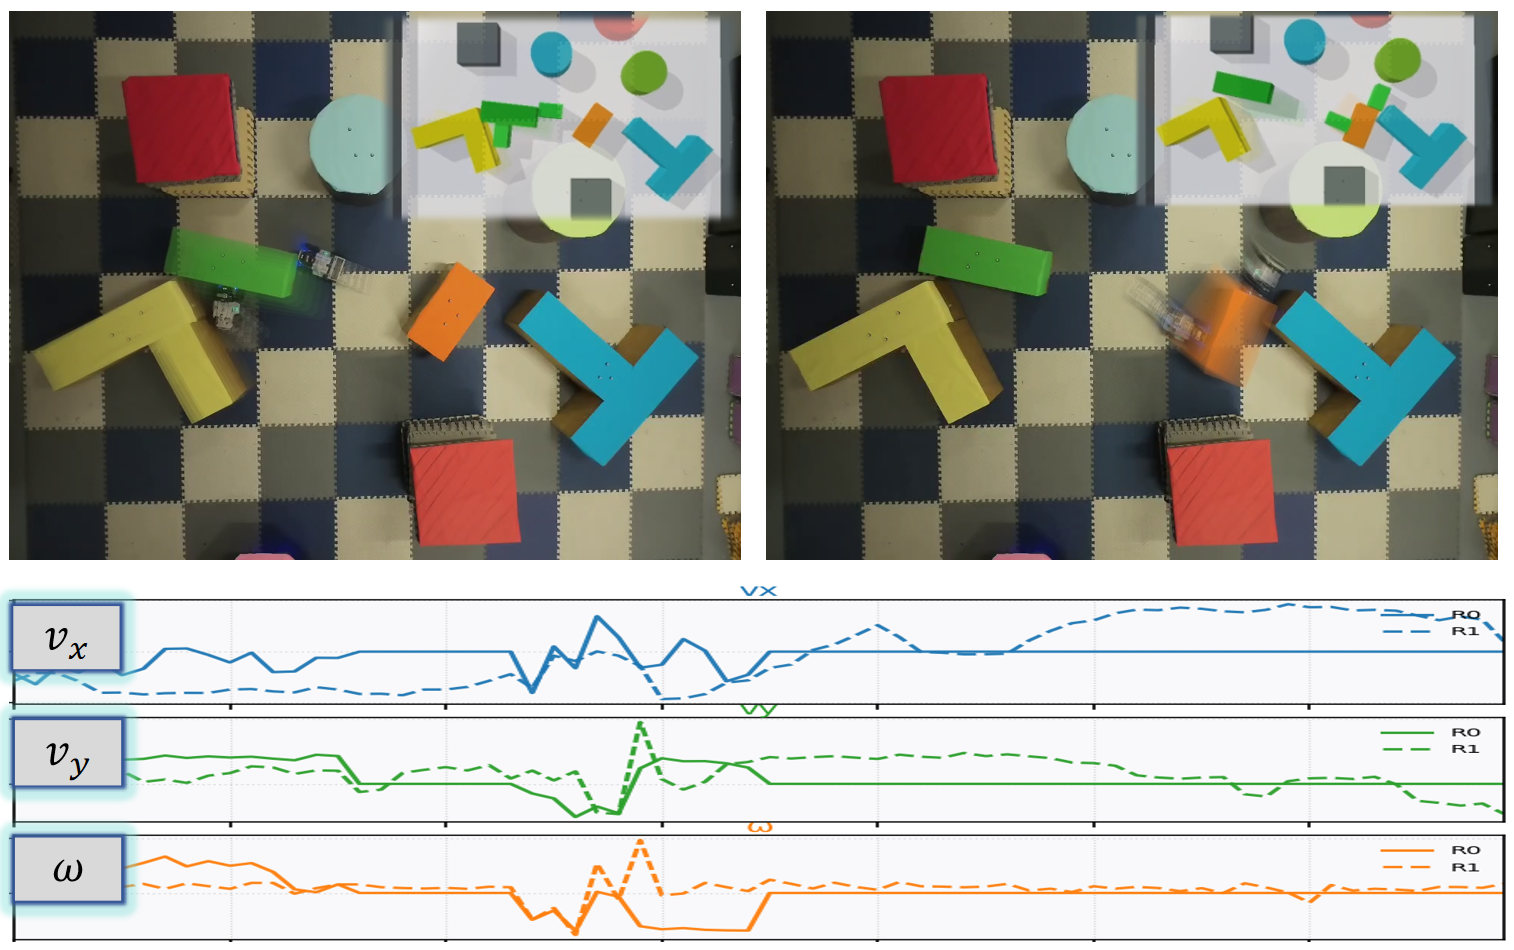
\includegraphics[width=\linewidth]{figures/hardware_snap.png}
%   \vspace{-2mm}
%   \caption{\textbf{Top:} two consecutive snapshots illustrating a chain push: R1 pushes an object, which then moves a neighbor. \textbf{Bottom:} velocity commands for both robots (\(v_x,v_y,\omega\)); the contact moment aligns with a brief rise in translational speed and differential angular commands.}
%   \label{fig:hardware_snap}
% \end{figure}